\chapter{Fluid-structure interaction}
\label{sec:fsi}
We model FSI with the developed CTVF scheme. This is advantageous since it can
eliminate the tensile instability issue in solid dynamics and ensure a homogeneous
particle distribution in fluids without any additional artificial stress terms.
We model FSI by the CTVF method, where both fluids and solid phases are modeled
using CTVF alone, while the interaction is modeled using a dummy particle
approach \citep{Adami2012}. We additionally consider the force acting on fluid
particles due to the interaction with the structure in the momentum equation. A
similar modification is carried out to the solid particle momentum equation as
well. The force is computed using a dummy particle approach of
\textcite{Adami2012}.


We study the deformation of the elastic plate due to the impact of water from a
dam break. The material properties of the elastic plate with a density of $2500$
kgm\textsuperscript{-3}, Young's modulus of $10^6$ Pa, and a Poisson ratio of
$0$. The material properties of the fluid are a density of 1000
kgm\textsuperscript{-3}, with no dynamic viscosity. In
\cref{fig:dam-breaking-onto-plate-snapshot}, we show the schematic of the
elastic dam break, and the deformed structure with fluid rise at a time instant.
\Cref{fig:water-impact-plate-deflection-quantitative} compares displacement of
the tip of the structure simulated with the current solver to other numerical
implementations. The current solver results are close to the other numerical
models.
\begin{figure}[tpb]
    \centering
  \begin{subfigure}{0.48\textwidth}
    \centering
    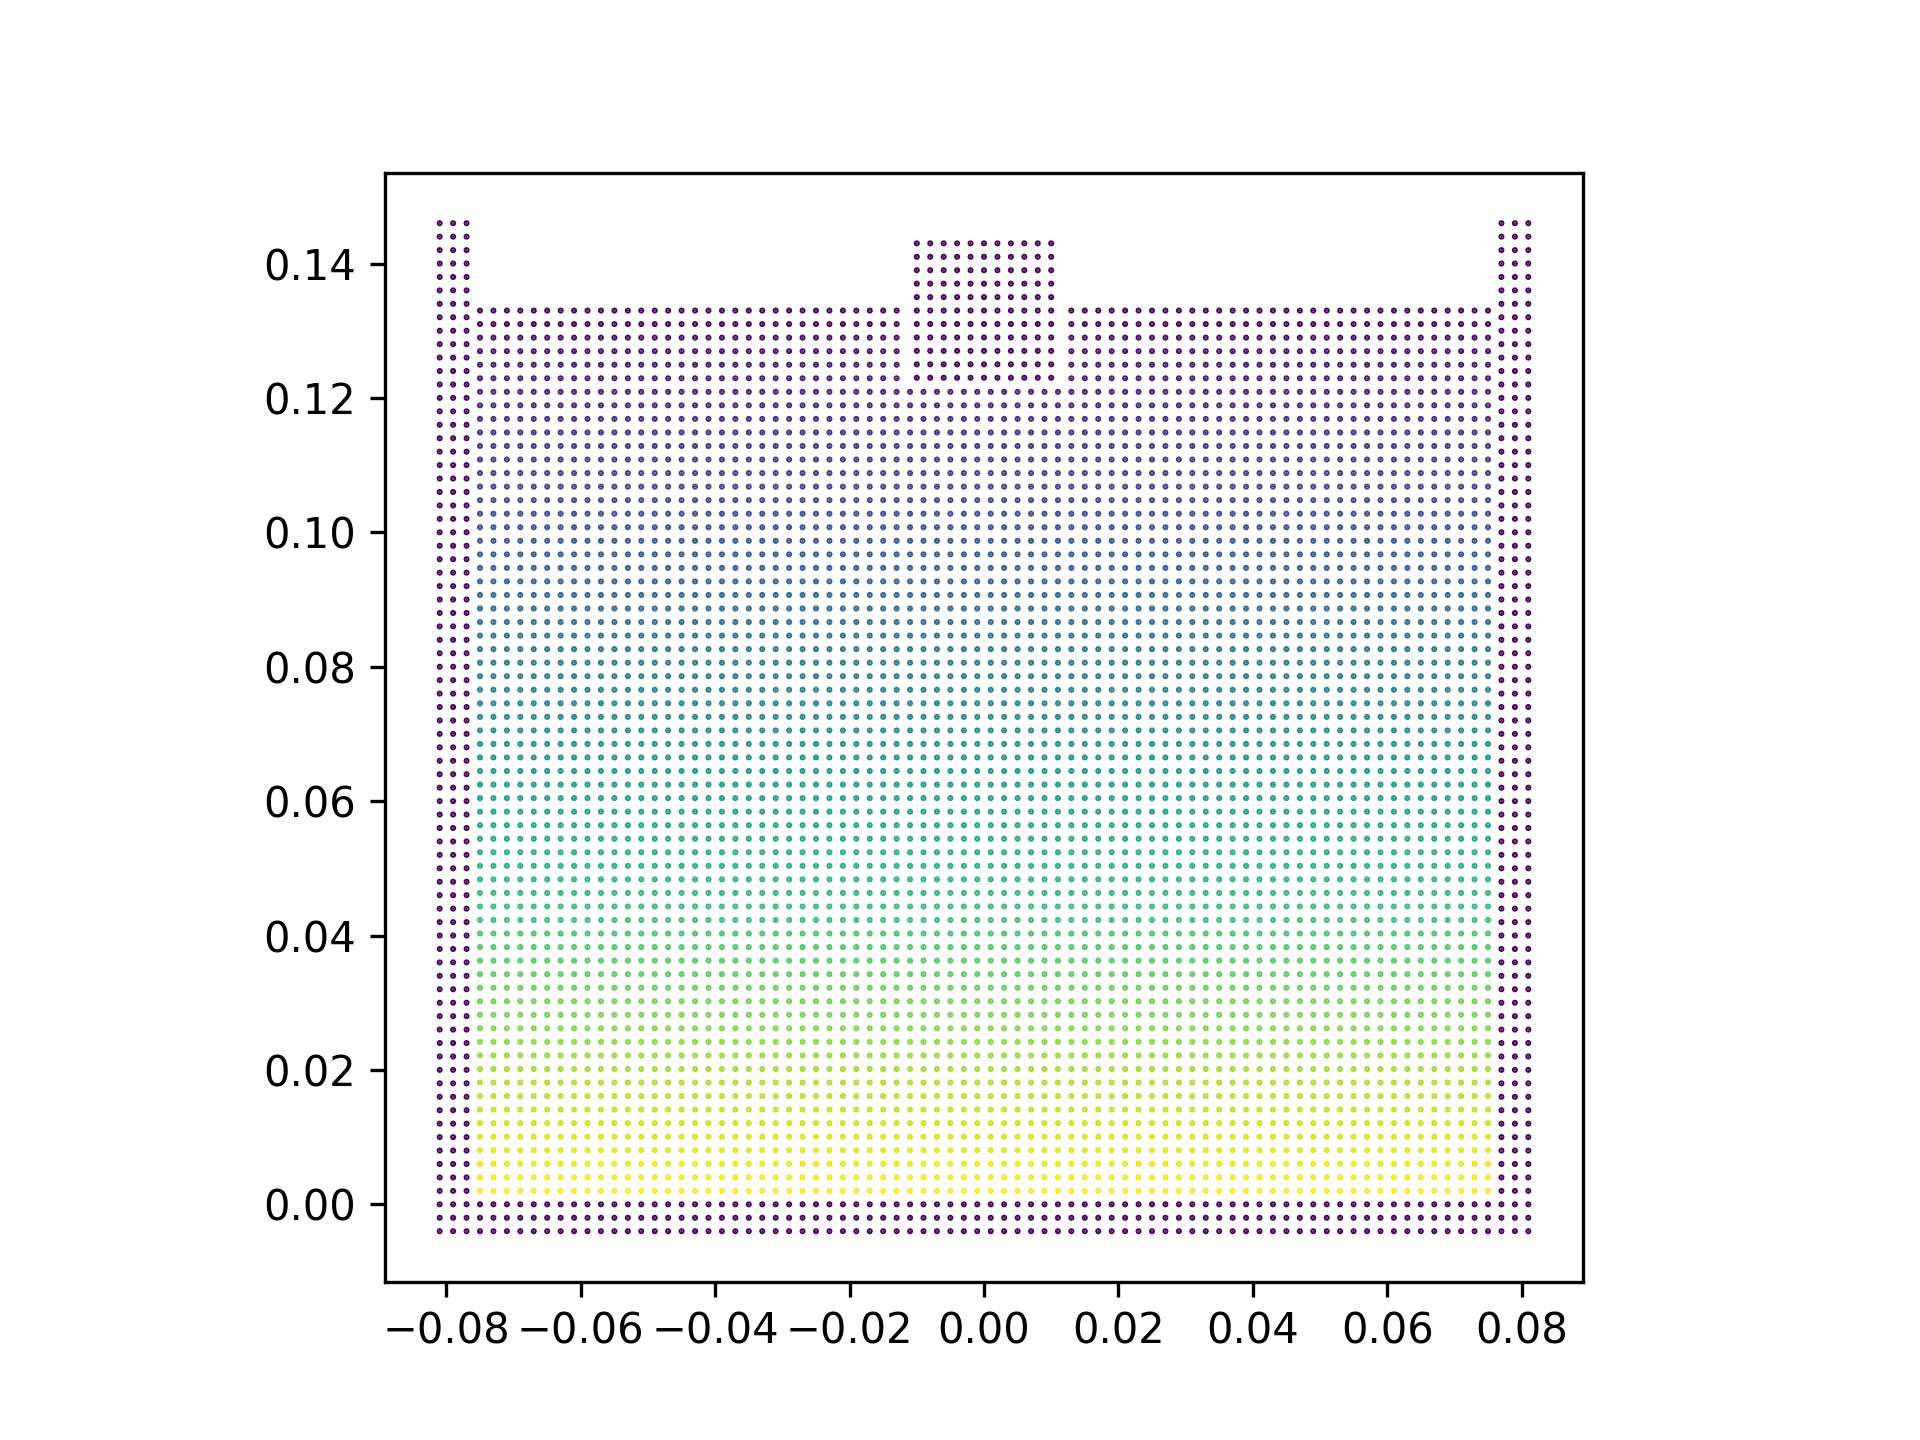
\includegraphics[scale=0.3]{images/fsi/images/sun_2019_dam_breaking_flow_impacting_an_elastic_plate/schematic}
    \caption{}
  \end{subfigure}
  \begin{subfigure}{0.48\textwidth}
    \centering
        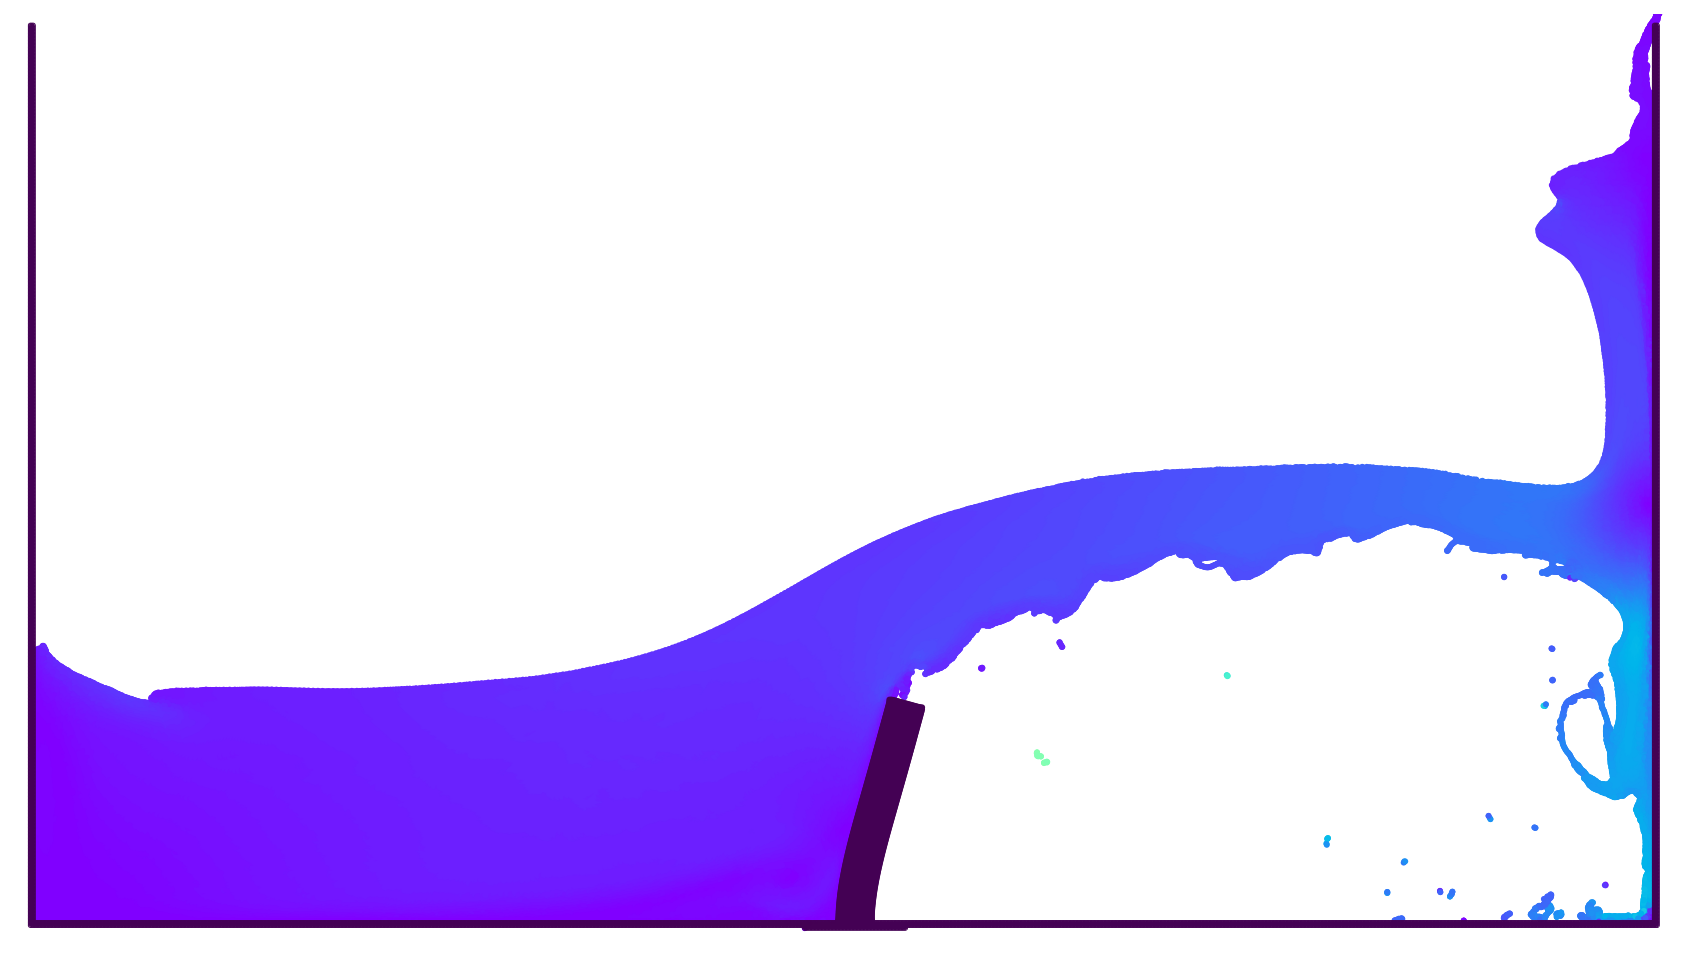
\includegraphics[scale=0.4]{figures/fsi/figures/sun_2019_dam_breaking_flow_impacting_an_elastic_plate/snap_t_2.png}
        \caption{}
  \end{subfigure}
    \caption
    { (a) Schematic of dam break flow over an elastic obstacle. (b) Snapshot of
      the deformed structure obstructing the fluid. }
    \label{fig:dam-breaking-onto-plate-snapshot}
\end{figure}
\begin{figure}[tpb]
  \centering
  \includegraphics[scale=0.45]{figures/fsi/figures/sun_2019_dam_breaking_flow_impacting_an_elastic_plate/x_amplitude}
  \caption{Time histories of horizontal displacement of the free end of the
    elastic structure compared against the numerical results of
    \citep{sun2019fully,bogaers2016evaluation}- Dam breaking flow impacting an
    elastic plate.}
\label{fig:water-impact-plate-deflection-quantitative}
\end{figure}
We have found that, the coupled CTVF solver is able to predict the deformation of the elastic
structure under hydrodynamics loads accurately.
